\documentclass[11pt,a4paper,twocolumn]{article}

%% ── Packages ──────────────────────────────────────────────────────────────
\usepackage[T1]{fontenc}
\usepackage[utf8]{inputenc}
\usepackage{mathptmx}
\usepackage[margin=1in,top=0.85in,bottom=1in]{geometry}
\usepackage{microtype}
\usepackage{booktabs}
\usepackage{amsmath}
\usepackage{xcolor}
\usepackage[hidelinks]{hyperref}
\usepackage{array}
\usepackage{tabularx}
\newcolumntype{Y}{>{\raggedright\arraybackslash}X}
\usepackage{caption}
\usepackage{graphicx}
\graphicspath{{figures/}{../figures/}}
\usepackage{titlesec}
\usepackage{dblfloatfix}
\usepackage{natbib}
\usepackage{fancyhdr}
\usepackage{tcolorbox}
\tcbuselibrary{skins,breakable}
\usepackage{algorithm}
\usepackage{algpseudocode}
\usepackage{listings}
\usepackage{mdframed}
\usepackage{float}
\usepackage{needspace}
\usepackage{enumitem}

%% Algorithm listing box (matches Algorithm~1 style)
\newtcolorbox{codealgobox}{
  colback=gray!6, colframe=gray!35, boxrule=0.4pt,
  arc=3pt, left=4pt, right=4pt, top=3pt, bottom=3pt
}
\newtcolorbox{metricbox}{
  colback=gray!6, colframe=gray!35, boxrule=0.4pt,
  arc=3pt, left=6pt, right=6pt, top=5pt, bottom=5pt,
  fontupper=\small
}

%% ── Layout ────────────────────────────────────────────────────────────────
\setlength{\columnsep}{0.25in}
\renewcommand{\arraystretch}{1.1}
\setlength{\tabcolsep}{4.5pt}
\captionsetup{font=small,labelfont=bf}

%% ── Section formatting ────────────────────────────────────────────────────
\titleformat{\section}{\normalfont\bfseries\large}{\thesection}{0.5em}{}
\titleformat{\subsection}{\normalfont\bfseries\normalsize}{\thesubsection}{0.5em}{}
\titleformat{\paragraph}[runin]{\normalfont\bfseries}{}{0em}{}[.\enspace]
\titlespacing{\section}{0pt}{7pt plus 2pt minus 2pt}{3pt}
\titlespacing{\subsection}{0pt}{5pt plus 2pt minus 2pt}{2pt}

%% ── Header ────────────────────────────────────────────────────────────────
\pagestyle{fancy}
\fancyhf{}
\rhead{\small\textit{TermPlanMT}}
\lhead{\small\textit{Kerins \& Abadour \textperiodcentered\ UPV/EHU}}
\cfoot{\thepage}
\renewcommand{\headrulewidth}{0.4pt}

%% ── Finding box ───────────────────────────────────────────────────────────
\newtcolorbox{finding}{
  enhanced, colback=gray!8, colframe=gray!40,
  boxrule=0.5pt, arc=2pt,
  left=4pt, right=4pt, top=3pt, bottom=3pt,
  fontupper=\small
}

%% ───────────────────────────────────────────────────────────────────────────
\title{\LARGE\bfseries TermPlanMT: Graph-Grounded Terminology Planning\\
for French--English Regulatory Medical Document Translation\\[4pt]
\large\normalfont When Ontology Grounding Helps and When It Does Not}

\author{
  Darragh Russell Kerins\\
  UPV/EHU\\
  \texttt{drussell001@ikasle.ehu.eus}
  \and
  Noumidia Abadour\\
  UPV/EHU\\
  \texttt{nabadour001@ikasle.ehu.eus}
}
\date{}

%% ═══════════════════════════════════════════════════════════════════════════
\begin{document}
\twocolumn[{%
  \maketitle
  \thispagestyle{fancy}
  \begin{tcolorbox}[
    colback=gray!5,
    colframe=gray!35,
    boxrule=0.5pt,
    arc=4pt,
    left=10pt, right=10pt, top=8pt, bottom=8pt,
    before skip=6pt,
    after skip=10pt,
    fontupper=\small
  ]
  \noindent\textbf{Abstract.}\enspace
  Terminology consistency is a critical quality dimension in the machine
  translation of regulatory medical documents, where mistranslated adverse
  event terms carry direct patient-safety consequences. We present
  \textbf{TermPlanMT}, a graph-augmented terminology-planning framework
  evaluated on a 126-segment French--English corpus drawn from a European
  Medicines Agency (EMA) Summary of Product Characteristics (SmPC). Six
  systems form an ablation ladder isolating the contributions of NER recall,
  MedDRA ontology grounding, and constrained decoding. Our central finding
  is that Concept Coverage Rate (CCR), the fraction of source spans grounded
  in a MedDRA ontology graph, is the binding constraint on terminology-aware
  MT: at 39\% CCR, graph-free systems (S1--S2) outperform all
  graph-augmented systems on fluency -- S1 leads on BLEU, S2 on chrF and
  Hypothesis--Reference Agreement (HRA) -- while improving NER quality yields
  $\approx$7~BLEU gains for graph-augmented Mistral systems (S3--S5-Mistral)
  but not for NLLB or S2. HTM scores the certified human reference at
  0.15--0.18, unchanged by full MedDRA alias expansion, confirming a
  structural mismatch between MedDRA nomenclature and professional
  translation practice. Ambiguous grounding causes the planning stage to
  abstain from locking critical terms, explaining why graph-augmented systems
  produce lower cross-document consistency than graph-free baselines.
  \end{tcolorbox}
  \vspace{6pt}
}]

%% ── Visual overview (systems + metric) ─────────────────────────────────────
\begin{figure*}[!t]
  \centering
  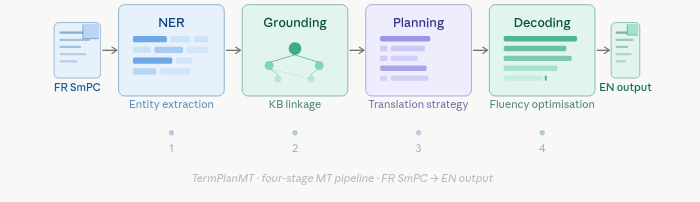
\includegraphics[width=\textwidth]{figure_pipeline_four_stage.png}
  \caption{Four-stage TermPlanMT pipeline (NER $\rightarrow$ grounding $\rightarrow$ planning $\rightarrow$ decoding).}
  \label{fig:pipeline}
\end{figure*}

%% ═══════════════════════════════════════════════════════════════════════════
\section{Introduction}
\label{sec:intro}

EMA Summaries of Product Characteristics (SmPCs) require a single
adverse-event concept to receive one identical English rendering across an
entire document--a requirement that affects pharmacovigilance signal detection
and patient safety \citep{neves2022evaluation}. Neural MT handles medical prose
fluently but is structurally indifferent to cross-segment consistency,
producing term drift (same source term, multiple renderings), concept
flattening (Lowest Level Term (LLT)-level terms collapsed to hypernyms), and coverage gaps
(multi-token spans outside NER). MedDRA's five-level hierarchy
(Table~\ref{tab:meddra}) provides validated English labels that are an
attractive grounding resource--if the grounding pipeline can cover enough of
the source text.

\noindent This paper makes the following contributions:

\begin{enumerate}[leftmargin=*, itemsep=4pt]

  \item \textbf{A six-system ablation ladder} that isolates the individual
  contributions of NER recall, MedDRA ontology grounding via Neo4j, and
  constrained decoding enforcement to terminology-aware MT quality.

  \item \textbf{Three novel evaluation metrics} -- HTM, rHTM, and HRA -- that
  measure terminology alignment at the ontology level rather than surface
  string overlap, with a diagnostic showing rHTM $\approx 0.15$--$0.18$ for
  certified human references.

  \item \textbf{A CCR bottleneck analysis} demonstrating that NER extraction
  quality, not retrieval or decoding strategy, is the primary constraint on
  graph-augmented MT performance.

  \item \textbf{A mechanistic consistency analysis} explaining the paradox in
  which graph-augmented systems produce lower cross-document term consistency
  than graph-free baselines, traced to the planning stage's
  abstain-on-ambiguity policy.

  \item \textbf{Reproducible artefacts} including per-segment HTM scores,
  bootstrap confidence intervals, and qualitative drift analysis exported as
  CSV and Markdown.

  \item \textbf{Two named phenomena}: the \textbf{register mismatch}
  (graph-augmented systems produce pharmacovigilance coding language while
  certified translators write clinical prose) and the \textbf{consistency
  paradox} (the most ontology-correct system is the least human-like and
  is never the preferred output in 30-segment human evaluation).

\end{enumerate}

%% ═══════════════════════════════════════════════════════════════════════════
\section{Related Work}
\label{sec:related}

Lexically constrained decoding \citep{hokamp2017lexically,post2018fast} and
terminology-aware training \citep{dinu2019training} enforce surface-level term
appearance but ignore ontological hierarchy and do not address candidate
selection when multiple levels are valid. \citet{herold2023improving} show that feeding long context directly into NMT
degrades output quality due to attention mechanism limitations, motivating our
pre-translation planning stage: rather than exposing the full document at decoding
time, we distil relevant terminology into a compact, structured prompt. \citet{labrak2024biomistral} release
BioMistral, the medically adapted LLM used for NER here.
\citet{neves2022evaluation} identify biomedical named entities broadly--diseases,
drugs, and procedures--as a persistent failure mode in biomedical MT. Our work
narrows this to the specific subtype of adverse event (AE) terminology as defined
by the MedDRA ontology, a distinction with direct regulatory consequences given
that AE terminology is legally standardised across EMA submissions. GraphRAG-style retrieval
\citep{edge2024local} into LLM prompts provides the template for our S3
system, adapting knowledge-grounded MT \citep{moussallem2019augmenting} to
a Neo4j MedDRA backend.

%% ═══════════════════════════════════════════════════════════════════════════
\section{Dataset}
\label{sec:data}

\paragraph{Corpus.}
Section~4.8 (Undesirable Effects) of the KEYTRUDA (pembrolizumab) SmPC
\citep{ema2024keytruda}: 126 aligned French--English segment pairs after
excluding segment~48\_028 (a dense frequency table whose n-gram overlap
distorts corpus metrics). Coverage: $\approx$4,400 words; all three failure
modes at high density.

\begin{table*}[t]
\centering
\footnotesize
\setlength{\tabcolsep}{5pt}
\renewcommand{\arraystretch}{1.15}
\caption{MedDRA hierarchy levels (MedDRA~v28) with acronym, meaning, and
specificity; examples follow the Section~4.8 immune-mediated pneumonitis chain.}
\label{tab:meddra}
\begin{tabularx}{\textwidth}{@{}c l
  >{\raggedright\arraybackslash\hsize=0.95\hsize}Y
  >{\raggedright\arraybackslash\hsize=0.75\hsize}Y
  >{\raggedright\arraybackslash\hsize=1.3\hsize}Y@{}}
\toprule
\textbf{Level} & \textbf{Abbr.} & \textbf{Meaning} & \textbf{Specificity} & \textbf{Example} \\
\midrule
L1 & SOC  & System Organ Class    & Broadest                  & Respiratory, thoracic and mediastinal disorders \\
L2 & HLGT & High Level Group Term & Broad                     & Lower respiratory tract inflammatory and immunologic conditions \\
L3 & HLT  & High Level Term       & Intermediate              & Pneumonitis and lung infiltration disorders \\
L4 & PT   & Preferred Term        & Specific clinical concept & Pneumonitis \\
L5 & LLT  & Lowest Level Term     & Most specific             & Immune-mediated pneumonitis \\
\bottomrule
\end{tabularx}
\end{table*}

\noindent
MedDRA (Medical Dictionary for Regulatory Activities) represents adverse events
using a five-level hierarchical terminology structure, enabling both
fine-grained clinical coding and higher-level safety aggregation. In our
corpus, adverse-event mentions map almost exclusively to L5 ($\approx$96\%).

\paragraph{Two NER conditions (zero-shot vs.\ QUAERO fine-tuned).}
\label{sec:ner_conditions}
We hold the MT stack (S1--S6) fixed and vary only how French spans are
extracted before Neo4j grounding. Both conditions use \textbf{BioMistral-7B}
\citep{labrak2024biomistral}; they differ in prompting versus supervised
adaptation on biomedical French NER.

\textbf{Condition A --- zero-shot prompting} (\texttt{ner\_biollm}):
BioMistral-7B in 4-bit inference with a French JSON-list prompt (no weight
updates). On the 126-segment evaluation set this yields CCR~=~39.0\% (184
grounded spans out of 472 extracted). The run also shows a systematic
prompting artefact: \textit{hypothyro\"{i}die} appears in 92/127 full-corpus
segments regardless of clinical content, which partially contaminates
cross-segment consistency scores for systems that consume these spans.

\textbf{Condition B --- Unsloth LoRA on QUAERO} (\texttt{ner\_biollm\_ft}):
the same base model fine-tuned with \textbf{Unsloth} on the \textbf{QUAERO}
French Medical corpus in BRAT format (EMEA + MEDLINE train splits;
\textbf{1{,}540} sentence-level training examples}; entity types DISO, CHEM, PROC only). Each sentence is an Alpaca instruction example
(extract disorders, drugs, and procedures as a JSON string list); training
uses 4-bit loading, LoRA rank~16 / $\alpha{=}32$ / dropout~0.05 on all
linear projections, 3~epochs, per-device batch~4, gradient accumulation~4,
learning rate $2{\times}10^{-4}$, cosine schedule, 10 warmup steps, and
response-only loss (\texttt{SFTTrainer}). Spans are written to
\texttt{segments\_ner\_unsloth\_full.jsonl} and fed through the identical
pipeline. On the evaluation set: 211 grounded spans out of 580 extracted
(CCR~=~36.4\%)\footnote{CCR depends on both NER recall and whether a span
exists in the MedDRA graph. Condition~B extracts more spans (580 vs.\ 472)
but grounds a larger share of difficult/rare strings, so the \emph{rate} can
fall while the absolute grounded count rises (211 vs.\ 184). Downstream
comparisons should treat CCR as a diagnostic, not as the manipulated variable.};
boundaries are cleaner and the hypothyroidism hallucination disappears.

Graph-augmented Mistral systems (S3--S5-Mistral) gain $\approx$7~BLEU only
under Condition~B (Table~\ref{tab:delta}), while S1/S2 translations are
unchanged. That pattern isolates \emph{span quality}---usable grounding and
clean boundaries---as the binding constraint upstream of graph retrieval, not
the graph machinery itself.

%% ═══════════════════════════════════════════════════════════════════════════
\section{System Architecture}
\label{sec:systems}

Six systems form an ablation ladder (Table~\ref{tab:systems}). S1--S5 share
the same four-stage pipeline: French NER $\rightarrow$ MedDRA grounding via
Neo4j $\rightarrow$ global terminology lock $\rightarrow$ MT decoding. S6 is a
glossary oracle ablation that replaces the MedDRA graph with a curated FR$\to$EN
glossary extracted from the reference translations.

\begin{table}[!ht]
\centering
\resizebox{\columnwidth}{!}{%
\small
\begin{tabular}{llllp{1.5cm}}
\toprule
\textbf{ID} & \textbf{Model} & \textbf{Graph} & \textbf{Enforce.} \\
\midrule
S1 & NLLB-200 600M      & No     & None   \\
S2 & Mistral-7B (doc)   & No     & None   \\
S3 & Mistral+GraphRAG   & Yes    & None   \\
S4 & S3 + reranking     & Yes    & Soft   \\
S5 & NLLB/Mistral+logit & Yes    & Hard   \\
S6 & NLLB + glossary    & Oracle & Hard   \\
\bottomrule
\end{tabular}}
\caption{Ablation ladder. S1 = NMT lower bound; S2 = LLM with full document
context; S3 is the key novel condition; S6 isolates term-source quality from
graph retrieval.}
\label{tab:systems}
\end{table}

\paragraph{Terminology planning.}
Before translation, \texttt{compute\_global\_locks()} scores each candidate
English rendering~$c$:
\begin{equation}
\text{Score}(c) = \alpha\,\text{Ctx}(c) + \beta\,\text{Nbr}(c)
               - \gamma\,\text{HP}(c)
\end{equation}
where Ctx is cosine similarity to source segments containing the term,
Nbr is similarity to adjacent MedDRA concept renderings, and
$\text{HP} = |\hat{d} - d_{\text{src}}|$ penalises wrong specificity level
($\alpha{=}0.5$, $\beta{=}0.3$, $\gamma{=}0.2$). When a term matches
\emph{multiple} MedDRA concepts, no lock is committed
(\S\ref{sec:consistency}).

\begin{algorithm}[t]
\caption{Global Terminology Planning -- \texttt{compute\_global\_locks}}
\label{alg:planning}
\begin{codealgobox}
\begin{lstlisting}[
  language=Python,
  basicstyle=\scriptsize\ttfamily,
  keywordstyle=\bfseries,
  commentstyle=\color{gray}\itshape,
  numbers=left,
  numberstyle=\tiny\color{gray},
  numbersep=4pt,
  xleftmargin=10pt,
  frame=none,
  showstringspaces=false,
  breaklines=true,
  columns=flexible
]
# Inputs: segments S, MedDRA graph G
# Weights: alpha=0.5, beta=0.3, gamma=0.2
# Output: lock map {fr_term -> en_rendering}

locks = {}
for fr_term in unique_ner_terms(S):
    concept = G.ground(fr_term)
    # exact match first, then fuzzy >= 90%

    if concept is None or G.is_ambiguous(fr_term):
        continue  # abstain: wrong lock propagates document-wide

    candidates = [concept.name] + G.neighbours(concept)
    best, best_score = None, -inf
    for r in candidates:
        ctx   = cosine(embed(segs), embed(r))
        nbr   = cosine(embed(r), embed(G.neighbours(concept)))
        hp    = abs(level(r) - level(concept))
        score = alpha*ctx + beta*nbr - gamma*hp
        if score > best_score:
            best, best_score = r, score
    locks[fr_term] = best

return locks
\end{lstlisting}
\end{codealgobox}
\end{algorithm}

The abstain-on-ambiguity policy (line 4) is a deliberate safety choice: when a French
term maps to multiple MedDRA concepts with equal confidence (e.g.\
\textit{pneumopathie inflammatoire} maps to both \textsc{Pneumonitis} and
\textsc{Interstitial Lung Disease}), forcing a lock risks propagating the wrong
concept across the entire document. The cost of this conservatism is reduced
cross-document consistency, since unlocked terms are resolved independently at
each segment by the decoder. We discuss this consistency paradox in
Section~\ref{sec:consistency}.

\paragraph{S5 -- Logit Boosting with Hard Fallback.}
S5 applies a two-layer decoding strategy. First, a soft logit bias
(\texttt{PhraseLogitBoost}, $\delta{=}1.75$ for NLLB, $\delta{=}1.25$ for
Mistral) increases the probability mass of tokens belonging to locked MedDRA
renderings without preventing the model from generating alternative phrasings
if contextually motivated. Second, for NLLB only, \texttt{force\_words\_ids}
enforces the locked phrase as a hard constraint via constrained beam search,
with automatic fallback to soft-only decoding if the constraint causes beam
failure. The Mistral variant uses soft boosting only, since instruction-tuned
LLMs are more sensitive to hard token forcing and exhibit greater fluency
degradation under strict constraints.

\subsection{MedDRA Knowledge Graph Construction}
\label{sec:graph-construction}

The grounding component $\mathcal{G}$ used throughout Algorithms~1--5 is a
Neo4j property graph built from the MedDRA v28 flat-file release, obtained
under academic licence via UPV/EHU.
Construction proceeds in four stages.

\paragraph{(1) Parsing the ASCII flat files.}
MedDRA distributes five pipe-delimited \texttt{*.asc} files.
The primary source is \texttt{mdhier.asc}, where each row encodes the
full SOC\,$\to$\,HLGT\,$\to$\,HLT\,$\to$\,PT\,$\to$\,LLT lineage for one
concept, together with English and French preferred labels.
A custom parser handles both the pipe-separated format (v28+) and the legacy
dollar-delimited format, with automatic encoding detection
(UTF-8\,$\to$\,CP1252\,$\to$\,ISO-8859-1).
This yields approximately 80,000 LLT records with complete five-level lineage.

\paragraph{(2) Building the French label index.}
The French MedDRA release is read in parallel to populate a
\texttt{fr\_label} property on each concept node.
After case-folding normalisation, 7{,}679 French surface forms are
\emph{ambiguous} --- a single normalised string maps to two or more distinct
MedDRA concepts (e.g., \textit{pneumopathie inflammatoire} resolves to both
\textsc{Pneumonitis} and \textsc{Interstitial Lung Disease}).
These keys are recorded in an \texttt{\_ambiguous} set and trigger the
abstain-on-ambiguity policy in \texttt{compute\_global\_locks}
(Algorithm~\ref{alg:planning}).

\paragraph{(3) Loading into Neo4j.}
Each MedDRA concept is stored as a \texttt{:Concept} node with properties
\texttt{\{id, name, fr\_label, level, tier\}}.
Parent--child relationships are represented as directed
\texttt{BROADER\_THAN} edges, producing a five-level DAG.
The graph is populated via batched Cypher \texttt{MERGE} transactions
against a Neo4j~5 Community instance deployed via Docker Compose.
The final graph contains \textbf{84{,}404 concept nodes} and
\textbf{91{,}082 entries} in the PT/LLT fuzzy index.

\paragraph{(4) Runtime API (\texttt{TermGraph}).}
All French concept keys are loaded into memory on first call (lazy,
cached).
String grounding applies exact case-fold matching first; if that fails,
RapidFuzz cosine similarity with a threshold of $\geq\!90\%$ is applied,
restricted to PT- and LLT-level nodes only (higher levels produce
over-generalised matches).
The \texttt{neighbours()} method returns concepts reachable via one or two
\texttt{BROADER\_THAN} hops; \texttt{same\_branch()} executes a
\texttt{shortestPath} Cypher query bounded to five hops.
A CCR diagnostic over the baseline NER condition confirms the grounding
ceiling: 23\% \textsc{Exact-Hit}, 11\% \textsc{Fuzzy-Hit}, 6\%
\textsc{Ambiguous}, and 60\% \textsc{Not-in-Graph} --- the last category
dominated by drug names, grade annotations, and numeric tokens that lie
outside the adverse-event subset of MedDRA indexed in the graph.

%% ═══════════════════════════════════════════════════════════════════════════
\section{Metrics}
\label{sec:metrics}

\needspace{26\baselineskip}
\begin{metricbox}
\noindent\textbf{Metric definitions.}
\begin{itemize}[noitemsep, topsep=3pt, leftmargin=*]
  \item \textbf{HTM} (Hierarchy-Aware Terminology Metric): per grounded
  NER span, score $= 1.0$ (exact MedDRA level), $0.5$ (same branch),
  $0.0$ (miss); macro-averaged (Algorithm~2).
  \item \textbf{rHTM} (Reference HTM): HTM applied to the certified human
  reference, not a system hypothesis. A dataset-level ceiling;
  values of $0.15$--$0.18$ confirm translators prefer phrasings outside
  the MedDRA preferred-term vocabulary.
  \item \textbf{HRA} (Hypothesis--Reference Agreement):
  $1 - |\mathrm{HTM}_\mathrm{hyp} - \mathrm{HTM}_\mathrm{ref}|$,
  macro-averaged (Algorithm~3). Measures agreement with professional
  translation practice rather than raw ontology proximity.
  \item \textbf{HTM-A} (Alias-Expanded HTM): accepts any ancestor up to
  SOC. Score invariance across tiers T1--T3 confirms failures are
  conceptual, not surface-level.
  \item \textbf{CCR} (Concept Coverage Rate): grounded spans / extracted
  spans. Identical across S1--S6 for a given NER condition; the primary
  diagnostic for NER quality.
\end{itemize}
\end{metricbox}

\begin{algorithm}[H]
\caption{HTM Scoring --- \texttt{compute\_htm}}
\label{alg:htm}
\begin{codealgobox}
\begin{lstlisting}[
  language=Python,
  basicstyle=\scriptsize\ttfamily,
  keywordstyle=\bfseries,
  commentstyle=\color{gray}\itshape,
  numbers=left,
  numberstyle=\tiny\color{gray},
  numbersep=4pt,
  xleftmargin=10pt,
  frame=none,
  showstringspaces=false,
  breaklines=true,
  columns=flexible
]
# Inputs: hypotheses H, segments S, graph G
# Output: macro-averaged HTM in [0, 1]

def htm_span(found, ref_label, ref_level, G):
    if not found: return 0.0
    node = G.get_by_name(found) or G.get_by_name(ref_label)
    if not node: return 0.0
    if node.level == ref_level: return 1.0      # exact tier
    if G.same_branch(found, ref_label): return 0.5
    return 0.0

scores = []
for row in H:
    hyp = row.hyp
    seg = S[row.id]
    for term in unique_ner_terms(seg):
        concept = G.ground(term, context=seg.fr)
        if concept is None: continue
        renderings = [concept.name] + G.candidates(concept)
        found = first_phrase_in(hyp, renderings)
        scores.append(htm_span(found, concept.name,
                              concept.level, G))
return mean(scores) if scores else 0.0
\end{lstlisting}
\end{codealgobox}
\end{algorithm}

\begin{algorithm}[H]
\caption{HRA --- \texttt{compute\_htm\_hyp\_vs\_ref}}
\label{alg:hra}
\begin{codealgobox}
\begin{lstlisting}[
  language=Python,
  basicstyle=\scriptsize\ttfamily,
  keywordstyle=\bfseries,
  commentstyle=\color{gray}\itshape,
  numbers=left,
  numberstyle=\tiny\color{gray},
  numbersep=4pt,
  xleftmargin=10pt,
  frame=none,
  showstringspaces=false,
  breaklines=true,
  columns=flexible
]
# Inputs: hypotheses H, segments S, graph G
# Output: mean agreement in [0, 1] (HRA)

agreements = []
for row in H:
    hyp, ref = row.hyp, seg.en_ref
    seg = S[row.id]
    for term in unique_ner_terms(seg):
        concept = G.ground(term, context=seg.fr)
        if concept is None: continue
        renderings = [concept.name] + G.candidates(concept)
        found_hyp = first_phrase_in(hyp, renderings)
        found_ref = first_phrase_in(ref, renderings)
        s_hyp = htm_span(found_hyp, concept.name,
                         concept.level, G)
        s_ref = htm_span(found_ref, concept.name,
                         concept.level, G)
        agreements.append(1.0 - abs(s_hyp - s_ref))
return mean(agreements) if agreements else nan
\end{lstlisting}
\end{codealgobox}
\end{algorithm}

\begin{algorithm}[H]
\caption{Soft Logit Boosting --- \texttt{PhraseLogitBoost}}
\label{alg:logit-boost}
\begin{codealgobox}
\begin{lstlisting}[
  language=Python,
  basicstyle=\scriptsize\ttfamily,
  keywordstyle=\bfseries,
  commentstyle=\color{gray}\itshape,
  numbers=left,
  numberstyle=\tiny\color{gray},
  numbersep=4pt,
  xleftmargin=10pt,
  frame=none,
  showstringspaces=false,
  breaklines=true,
  columns=flexible
]
# Inputs: tokenizer tok, locked phrases P, boost delta
# Applied each decoding step to logits vector scores

class PhraseLogitBoost(LogitsProcessor):
    def __init__(self, tok, phrases, boost=1.75):
        self.boost = boost
        self.ids = set()
        for p in phrases:
            for tid in tok(p, add_special_tokens=False).input_ids:
                self.ids.add(tid)

    def __call__(self, input_ids, scores):
        for tid in self.ids:
            if 0 <= tid < scores.shape[-1]:
                scores[:, tid] += self.boost
        return scores
# S5-NLLB: delta=1.75; S5-Mistral: delta=1.25
\end{lstlisting}
\end{codealgobox}
\end{algorithm}

\begin{algorithm}[H]
\caption{Hard Phrase Locking --- \texttt{force\_words\_ids} (NLLB S5/S6)}
\label{alg:force-words}
\begin{codealgobox}
\begin{lstlisting}[
  language=Python,
  basicstyle=\scriptsize\ttfamily,
  keywordstyle=\bfseries,
  commentstyle=\color{gray}\itshape,
  numbers=left,
  numberstyle=\tiny\color{gray},
  numbersep=4pt,
  xleftmargin=10pt,
  frame=none,
  showstringspaces=false,
  breaklines=true,
  columns=flexible
]
# Inputs: segment seg, lock map L, graph G
# Output: constrained NLLB translation

phrases = []
for term in seg.terms:
    concept = G.ground(term, context=seg.fr)
    if concept is None: continue
    en = L.get(term) or concept.name
    phrases.append(en)

phrase_ids = [tok(p, add_special_tokens=False).input_ids
              for p in phrases if p]
beams = min(10, 5 + len(phrases))
try:
    out = model.generate(
        **encode(seg.fr),
        logits_processor=[PhraseLogitBoost(tok, phrases)],
        force_words_ids=phrase_ids,
        num_beams=beams, max_new_tokens=256)
except BeamSearchFailure:
    # fallback: soft boost only (no hard lock)
    out = model.generate(..., logits_processor=[boost])
return decode(out)
\end{lstlisting}
\end{codealgobox}
\end{algorithm}

\noindent Fluency: corpus BLEU \citep{papineni2002bleu} and chrF\texttt{++}
\citep{popovic2017chrf} via SacreBLEU; neural: COMET \citep{rei2020comet}.
HTM-A extends HTM matching across three tiers: T1 exact LLT; T2 adds Preferred
Term (PT) parent; T3 adds all same-branch ancestors.

\paragraph{CCR and drift.}
CCR~$=$~grounded/extracted spans; identical across S1--S6 for a given NER
condition. Term drift~$= (D-1)/(N-1)$ for $D$ distinct renderings across
$N$ segments; drift~$=0$ is perfect consistency.

%% ═══════════════════════════════════════════════════════════════════════════
\section{Results}
\label{sec:results}

\subsection{Main Results}

\begin{table}[!ht]
\centering
\footnotesize
\setlength{\tabcolsep}{3pt}
\begin{tabular}{lrrrrr}
\toprule
System & BLEU & chrF\texttt{++} & COMET & HTM & HRA \\
\midrule
S1 NLLB       & \textbf{22.89} & 37.14 & \textbf{0.639} & 0.321 & 0.672 \\
S2 Mistral    & 22.51 & \textbf{39.95} & 0.637 & 0.413 & \textbf{0.743} \\
S3 GraphRAG   & 10.39 & 34.36 & 0.586 & 0.397 & 0.601 \\
S4 rerank     &  9.93 & 34.24 & 0.583 & \textbf{0.429} & 0.579 \\
S5 NLLB+boost & 21.59 & 35.91 & 0.638 & 0.353 & 0.661 \\
S5 Mist+boost & 10.32 & 34.32 & 0.585 & 0.380 & 0.607 \\
S6 NLLB+gls\textsuperscript{$\star$} & 20.00 & 35.11 & 0.634 & 0.321 & 0.694 \\
\midrule
Reference     & --   & --   & --   & 0.151 & 1.000 \\
\bottomrule
\end{tabular}
\caption{Baseline NER condition (\texttt{ner\_biollm}, CCR~=~39.0\%;
126~segments, 48\_028 excluded). BLEU/chrF\texttt{++} via SacreBLEU;
COMET via wmt22-comet-da; HTM/HRA from Neo4j.
\textsuperscript{$\star$}S6 is a glossary oracle (terms from reference).}
\label{tab:biollm}
\end{table}

\begin{table}[!ht]
\centering
\footnotesize
\setlength{\tabcolsep}{3pt}
\begin{tabular}{lrrrrr}
\toprule
System & BLEU & chrF\texttt{++} & COMET & HTM & HRA \\
\midrule
S1 NLLB         & 22.89 & 37.14 & \textbf{0.639} & 0.550 & 0.429 \\
S2 Mistral      & \textbf{22.51} & \textbf{39.95} & 0.637 & \textbf{0.735} & \textbf{0.476} \\
S3 GraphRAG\textsuperscript{†} & 19.58 & 35.33 & 0.626 & 0.664 & 0.440 \\
S4 rerank\textsuperscript{†}   & 19.66 & 35.36 & 0.626 & 0.664 & 0.450 \\
S5 NLLB+boost   & 21.37 & 36.06 & 0.637 & 0.578 & 0.403 \\
S5 Mist+boost\textsuperscript{†} & 20.61 & 35.78 & 0.626 & 0.673 & 0.450 \\
S6 NLLB+gls\textsuperscript{$\star$} & 20.09 & 34.81 & 0.632 & 0.536 & 0.408 \\
\midrule
Reference       & --   & --   & --   & 0.178 & 1.000 \\
\bottomrule
\end{tabular}
\caption{Fine-tuned NER condition (\texttt{ner\_biollm\_ft};
CCR~=~36.4\%; 126 segments, 48\_028 excluded).
\textsuperscript{†}Contamination-filtered (18/127 rows scored as empty hyps).
\textsuperscript{$\star$}S6 uses a glossary oracle from the reference.}
\label{tab:finetuned}
\end{table}

\noindent
Tables~\ref{tab:biollm} and~\ref{tab:finetuned} report corpus-level scores;
Fig.~\ref{fig:metrics-grouped} visualises the same systems (baseline BioMistral
NER left, fine-tuned NER right). Under fine-tuned NER, graph-augmented Mistral
systems close the fluency gap substantially, confirming NER quality as the
binding constraint.

\begin{figure*}[!ht]
\centering
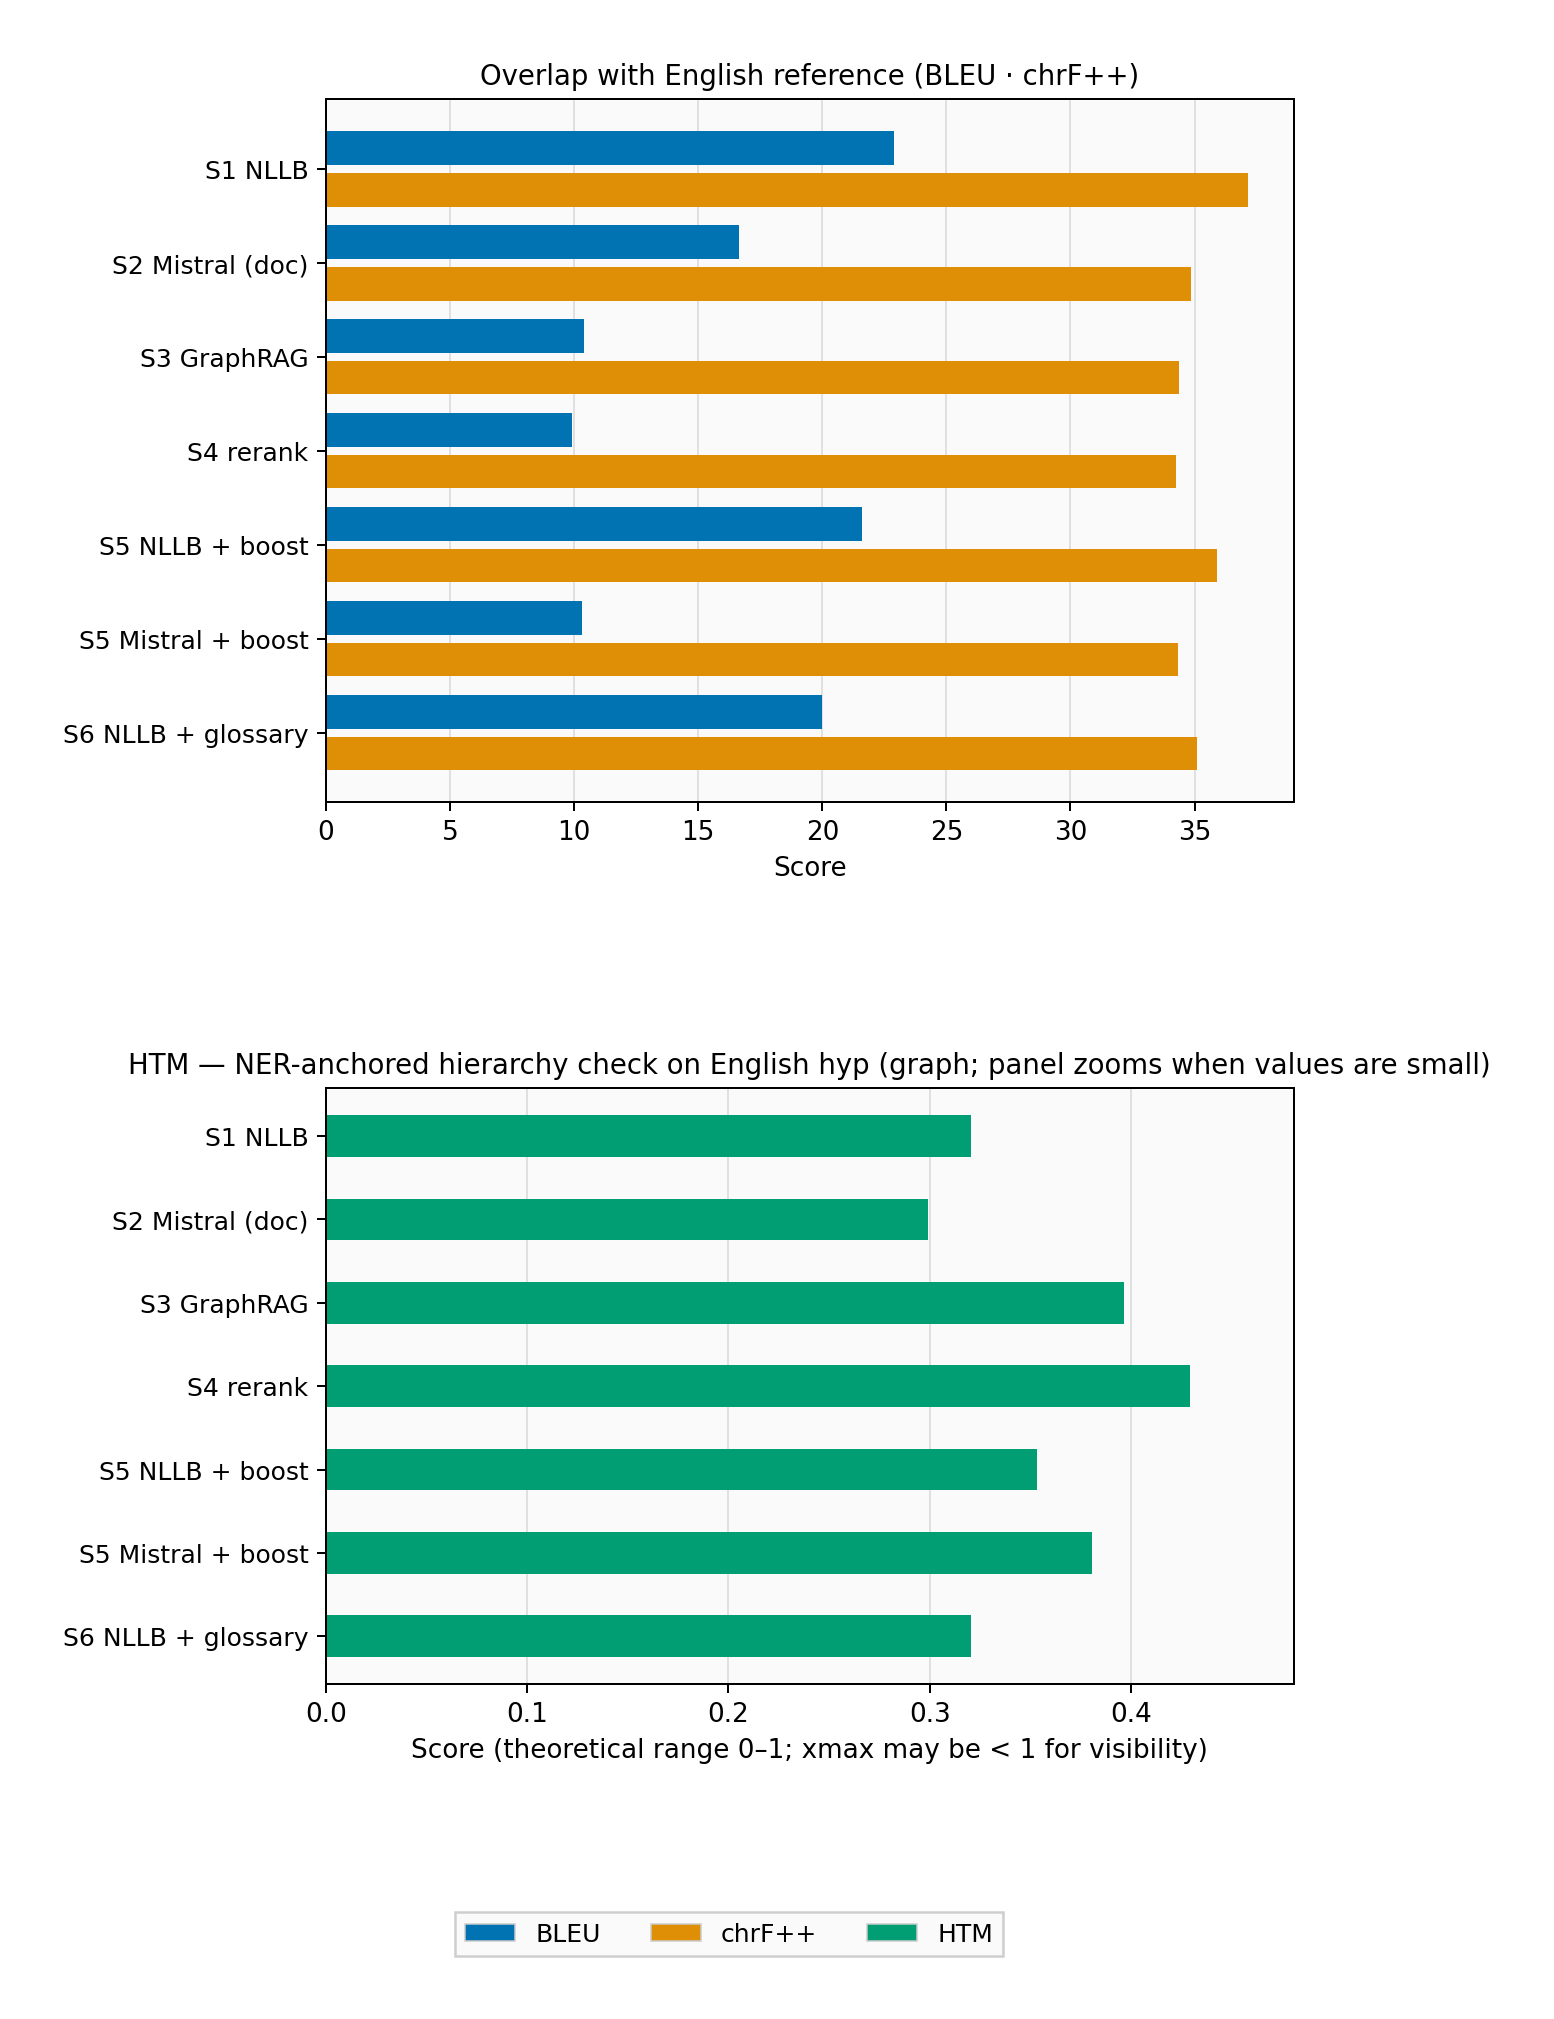
\includegraphics[width=0.47\textwidth]{comparison_metrics_grouped_baseline.png}\hfill
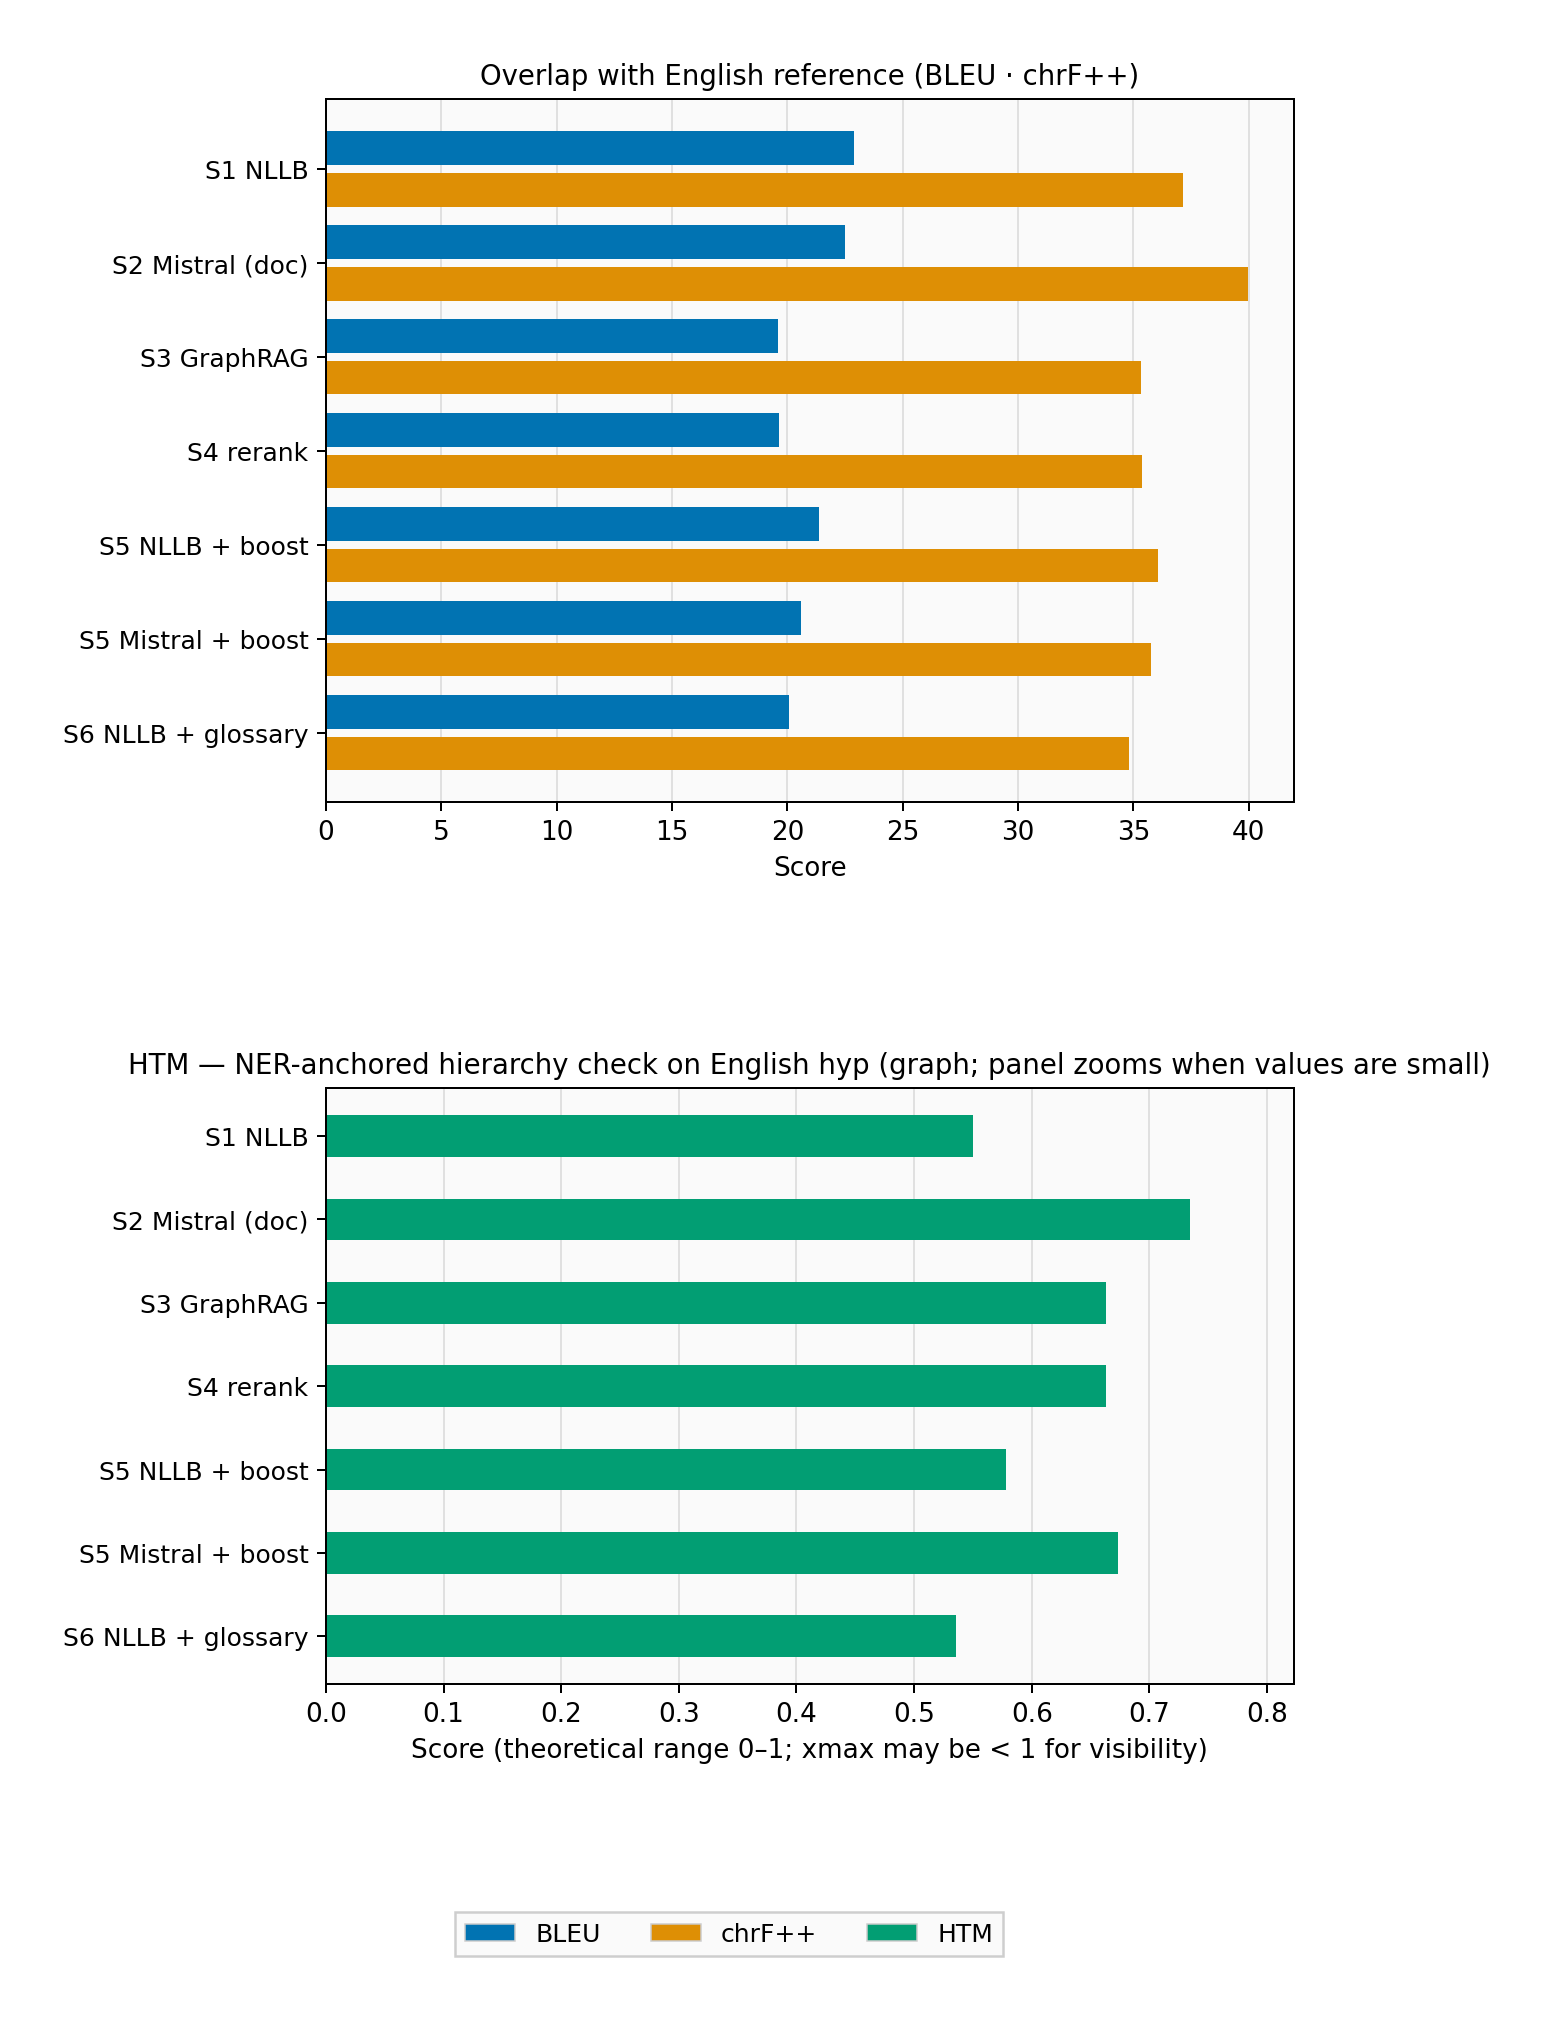
\includegraphics[width=0.47\textwidth]{comparison_metrics_grouped_finetuned.png}
\caption{Grouped metrics by system. \textbf{Left:} baseline NER
(\texttt{ner\_biollm}, CCR~=~39.0\%). \textbf{Right:} fine-tuned NER
(\texttt{ner\_biollm\_ft}, CCR~=~36.4\%). Top: BLEU and chrF\texttt{++};
bottom: HTM (lexical, graph-aware). HTM is not comparable across panels.}
\label{fig:metrics-grouped}
\end{figure*}

\paragraph{HTM is recall-dependent on NER quality.}
BLEU and chrF scores for S1 and S2 are identical across both NER conditions
(Tables~\ref{tab:biollm} and~\ref{tab:finetuned}), confirming that the
underlying translations did not change. However, HTM scores shift substantially:
S1 HTM rises from $0.321$ to $0.550$ and S2 from $0.413$ to $0.735$ under
fine-tuned NER. This is a \emph{metric artifact}, not a translation improvement.
HTM is computed only over spans the NER model successfully extracts; a stronger
NER model exposes a larger and more challenging set of terminology spans,
changing both the denominator and the matched set simultaneously. Scores across
NER conditions are therefore not directly comparable and should be interpreted
within each condition only. Fig.~\ref{fig:tradeoff} shows the chrF\texttt{++}/HTM
scatter \emph{within} each NER condition (separate axes; do not compare HTM
across panels).

\begin{figure*}[!ht]
\centering
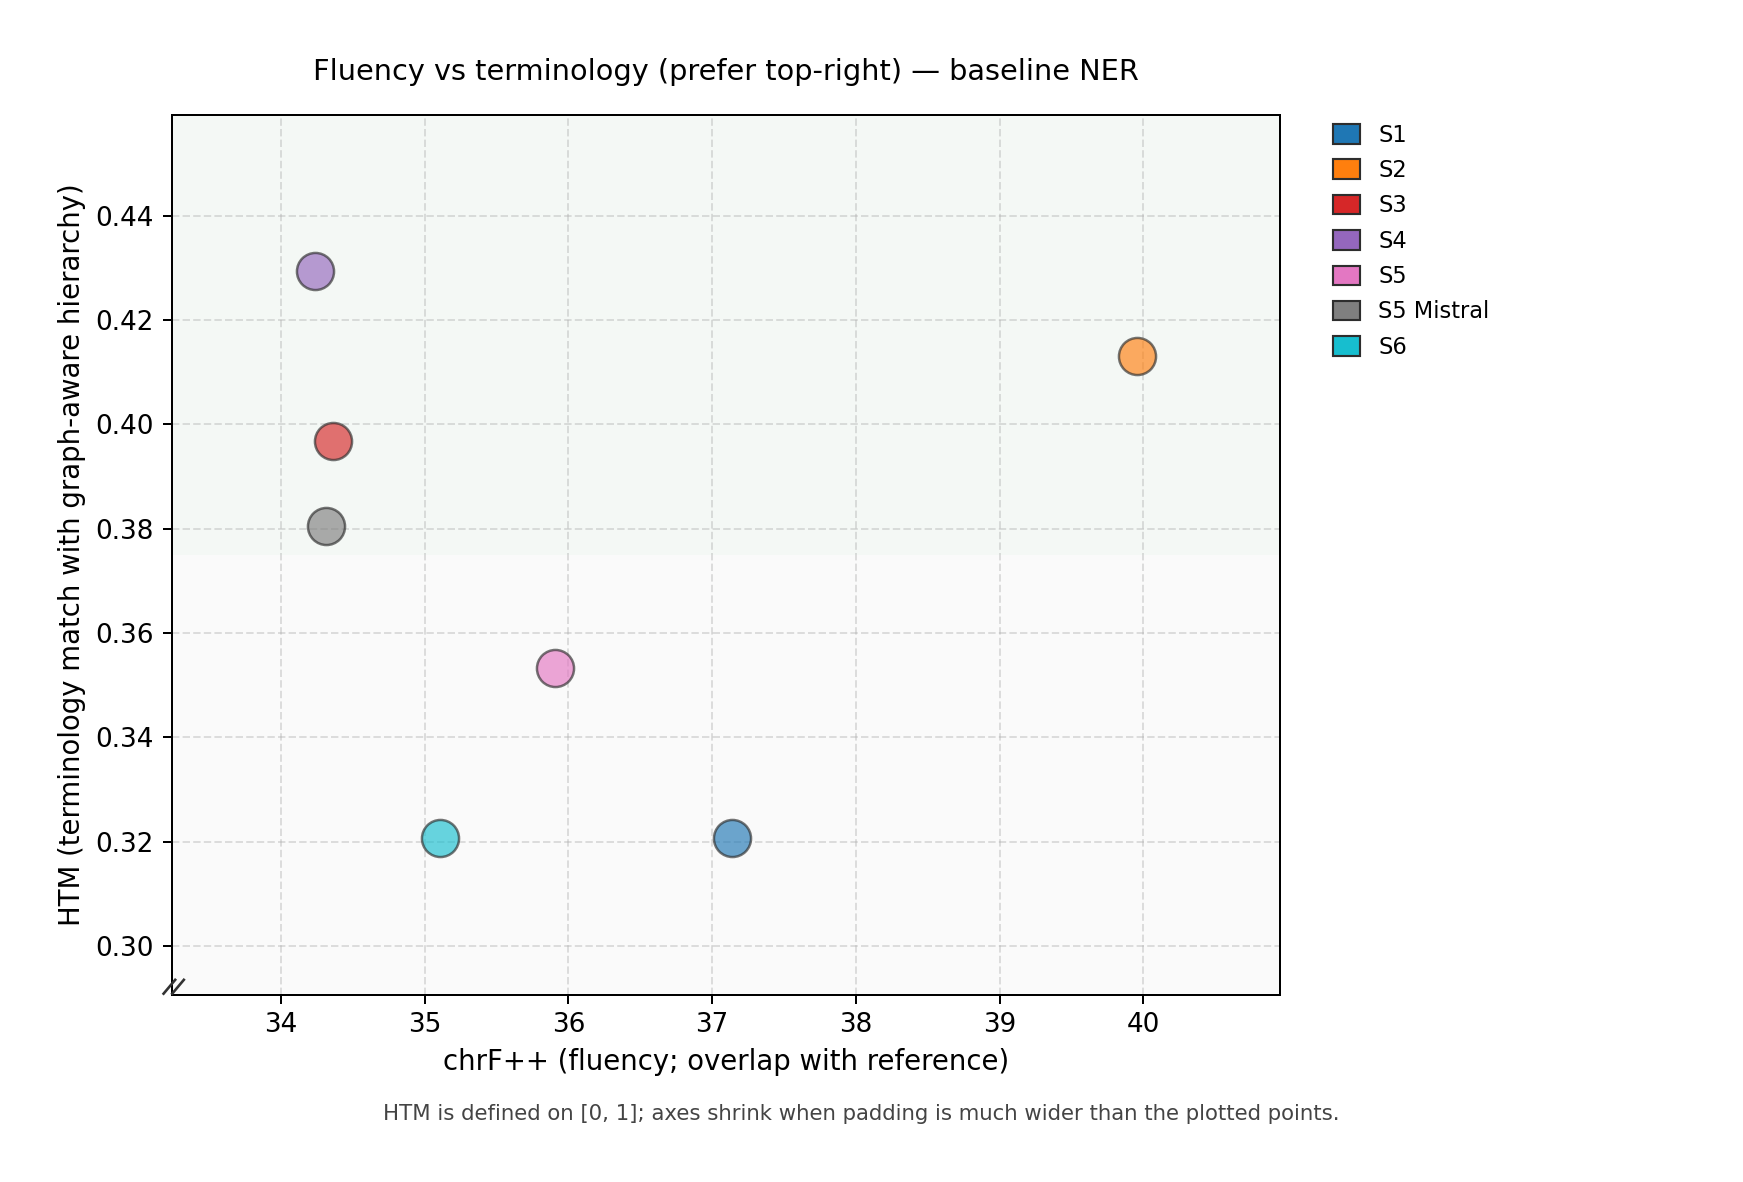
\includegraphics[width=0.47\textwidth]{comparison_tradeoff_chrF_vs_HTM_baseline.png}\hfill
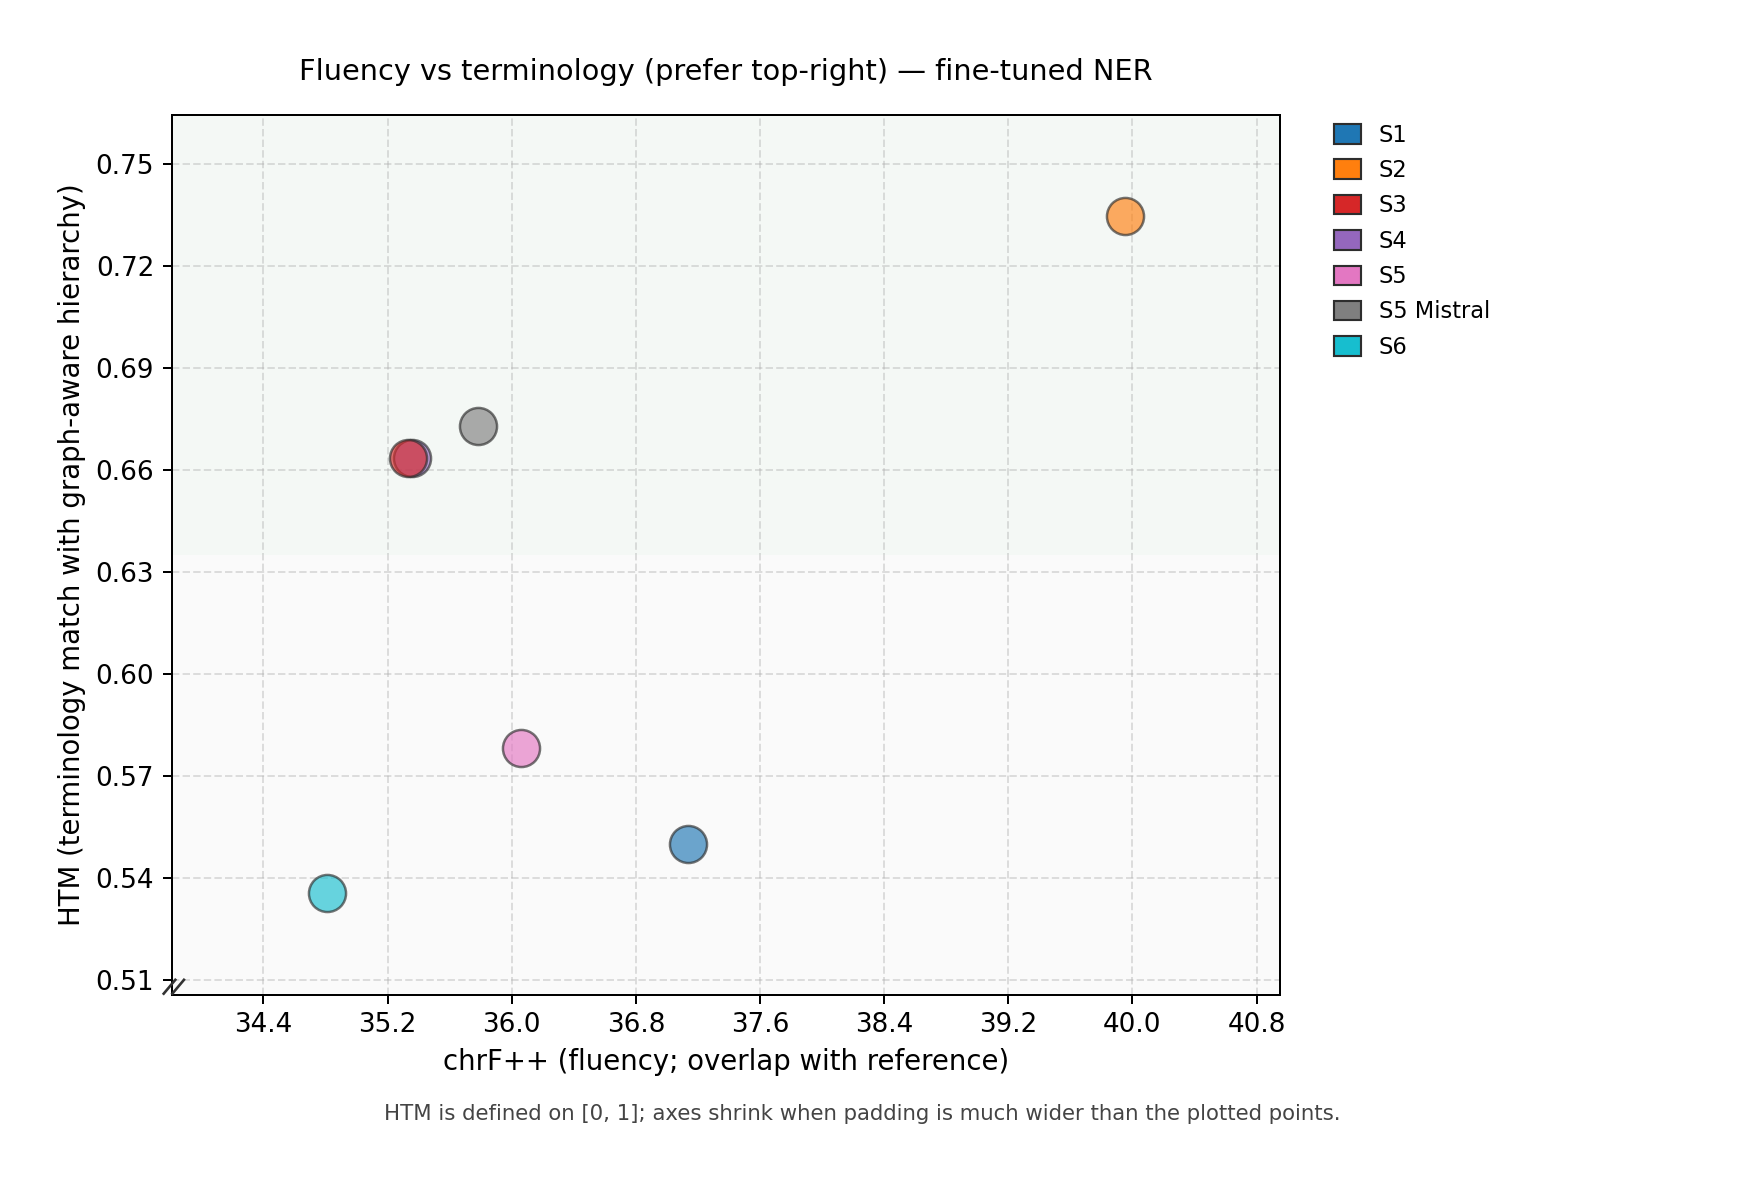
\includegraphics[width=0.47\textwidth]{comparison_tradeoff_chrF_vs_HTM_finetuned.png}
\caption{chrF\texttt{++} vs.\ HTM trade-off by system.
\textbf{Left:} baseline NER (\texttt{ner\_biollm}).
\textbf{Right:} fine-tuned NER (\texttt{ner\_biollm\_ft}).
HTM uses different grounded span sets in each panel; interpret fluency--terminology
trade-offs only within a panel.}
\label{fig:tradeoff}
\end{figure*}

\subsection{CCR is the Binding Constraint}
\label{sec:ccr_bottleneck}

Table~\ref{tab:delta} isolates the effect of NER quality by holding all other
pipeline components fixed and comparing the same system across NER conditions.

\begin{table}[!ht]
\centering
\footnotesize
\setlength{\tabcolsep}{3pt}
\begin{tabular}{lrrl}
\toprule
System & $\Delta$BLEU & $\Delta$chrF\texttt{++} & 95\% CI $\Delta$BLEU \\
\midrule
S1 NLLB        & $\pm$0.00 & $\pm$0.00 & $[$0.00,\,0.00$]$ \\
S2 Mistral\textsuperscript{$\ddagger$} & $\pm$0.00 & $\pm$0.00 & $[$0.00,\,0.00$]$ \\
S3 GraphRAG    & \textbf{+7.07} & +0.97 & $[$+1.07,\,+11.10$]$ \\
S4 rerank      & \textbf{+7.42} & +1.12 & $[$+1.18,\,+11.53$]$ \\
S5 NLLB+boost  & $-$0.16 & +0.15 & $[$$-0.98$,\,+0.66$]$ \\
S5 Mist+boost  & \textbf{+7.16} & +1.46 & $[$+1.10,\,+11.66$]$ \\
S6 NLLB+gls\textsuperscript{$\star$}   & +0.09 & $-$0.30 & -- \\
\bottomrule
\end{tabular}
\caption{Paired gain (fine-tuned minus baseline NER) on 126~segments.
$\Delta$BLEU is the paired bootstrap estimate (2{,}000 resamples, seed~42);
95\% CIs for S3--S5-Mistral exclude~0.
$\Delta$chrF\texttt{++} is the corpus-level paired difference.
\textsuperscript{$\ddagger$}S2 shares the same inference JSONL across conditions.
\textsuperscript{$\star$}S6 CI not computed (oracle glossary).}
\label{tab:delta}
\end{table}

\begin{finding}
S1 is unchanged (no graph). S2 is exactly zero: the same inference JSONL is
shared across both NER conditions, so $\Delta$BLEU is zero by construction.
S3--S5-Mistral show $\approx$7-point $\Delta$BLEU with intervals strictly
above zero, isolating the NER bottleneck on the graph path. S5-NLLB is
effectively flat. The S6 oracle glossary yields negligible gain, showing
that logit boosting with reference-extracted terms does not improve over
the graph path once NER quality is matched.
\end{finding}

The 95\% paired bootstrap confidence intervals for the BLEU gain of fine-tuned
graph-augmented Mistral systems (S3--S5-Mistral) over their baseline-NER
counterparts exclude zero (see Table~\ref{tab:delta}), confirming statistical
significance at $p < 0.05$. Graph-free systems (S1, S2) and S5-NLLB show
confidence intervals that include zero, indicating their apparent gains are not
reliably distinguished from noise.

S1 leads on corpus BLEU and S2 leads on chrF and HRA in the baseline NER
condition (Table~\ref{tab:biollm}): graph-augmented systems fall well below
both because the graph covers fewer than 40\% of source spans while injected
MedDRA strings hurt fluency in segments where it is active. S2's lead on HRA
(0.743) reflects the human-like output of full-document Mistral context without
graph interference. The contrast between zero $\Delta$BLEU for S1, S2, and
S5-NLLB versus large $\Delta$BLEU for S3--S5-Mistral isolates the bottleneck
upstream of graph retrieval. Higher NER coverage would likely close the S2/S3
fluency gap.

A post-hoc CCR diagnostic (\texttt{tools/ccr\_diagnostic.py}) classifying the
171 unique baseline NER terms against the Neo4j graph found that 60\% are absent
from MedDRA entirely (\textsc{not\_in\_graph}), compared to 54\% of the 246
fine-tuned terms; a further 6--8\% are ambiguous (multiple concept matches,
triggering the planner's abstain policy), and only 23--32\% ground via exact
string match. The dominant not-in-graph category is populated by non-medical
tokens (\textit{pembrolizumab}, grade annotations, numeric ranges) that NER
extracted as candidate spans but that have no MedDRA equivalent -- confirming
that the CCR ceiling is set by NER precision, not by graph coverage gaps.

\subsection{Missing Terms, Flattening, and Consistency}

Under baseline NER, S5-Mistral achieves the lowest missing-term rate;
S1-NLLB misses the majority of grounded terms. Zero concept flattening
events are observed for grounded L5 source terms, partly an evaluation
artefact that HTM-A addresses. Cross-document modal agreement is highest
for graph-free systems under baseline NER (S1: 0.993, S2: 0.984, S3: 0.946);
under fine-tuned NER the gap narrows (S3: 0.976) but S2 (0.985) remains
the most consistent Mistral system, confirming that the consistency
advantage of S1-NLLB is a vocabulary artefact rather than terminological reasoning.

%% ═══════════════════════════════════════════════════════════════════════════
\section{The HTM--Practice Gap}
\label{sec:htm_gap}

\subsection{Why the Reference Scores Near Zero}

On the baseline NER manifest, rHTM~$= 0.151$ on the professional reference
(Table~\ref{tab:biollm}); under fine-tuned NER the reference HTM is 0.178
(Table~\ref{tab:finetuned}) because the grounded span set differs.
In both cases the score stays below several MT systems on HTM. Professional
translators do not transcribe MedDRA LLT strings verbatim: the LLT
\textit{Immune-mediated pneumonitis} appears as \textit{pneumonitis} in
tabular contexts and as \textit{immune-related pneumonitis} in descriptive
contexts.

\subsection{Alias Expansion Does Not Close the Gap}

\begin{table}[!ht]
\centering
\small
\begin{tabular}{lp{3.5cm}rr}
\toprule
Tier & Accepts & Low & Hi \\
\midrule
T1 & Exact LLT           & 0.151 & 0.178 \\
T2 & T1 + PT parent      & 0.151 & 0.178 \\
T3 & T2 + branch ancestors & 0.151 & 0.178 \\
\bottomrule
\end{tabular}
\caption{rHTM-A on the professional reference under three alias tiers (Low =
baseline NER manifest; Hi = fine-tuned NER manifest). All tiers yield
identical scores within each manifest.}
\label{tab:aliases}
\end{table}

\begin{finding}
The ancestor chain for \textit{pneumopathie inflammatoire} contains
\textit{pneumonitis}, so the null T1$\to$T3 delta is not a graph coverage
gap. Professional translators use phrasings such as \textit{immune-related
pneumonitis} and \textit{inflammatory lung disease} that lie entirely outside
the MedDRA preferred-label tree at any level. The mismatch is structural:
MedDRA labels are designed for pharmacovigilance coding, not regulatory prose.
\end{finding}

HTM should therefore be interpreted as a measure of MedDRA-proximity, not
translation quality. The HRA column is the complementary measure. Notably,
graph-augmented systems score consistently \emph{lower} on HRA than S2
(Table~\ref{tab:biollm}: S3~=~0.601 vs.\ S2~=~0.743;
Table~\ref{tab:finetuned}: S3~=~0.440 vs.\ S2~=~0.476): the graph pushes
outputs toward MedDRA labels that professional translators avoid.
The fluency--terminology trade-off is in Fig.~\ref{fig:tradeoff}; per-system
inference times are in the project repository (\texttt{results/ner\_biollm/figures/}).

%% ═══════════════════════════════════════════════════════════════════════════
\section{Consistency Failure Analysis}
\label{sec:consistency}

\paragraph{Term drift (qualitative).}
\textit{Pneumopathie inflammatoire} occurs in four baseline segments where it
is grounded for S3/S4/S5-Mistral, and in eight fine-tuned segments (more NER
hits for the same French string). Those systems emit two renderings--often
\textit{pneumonitis} in incidence-style sentences and \textit{immune-mediated
pneumonitis} elsewhere--yielding drift scores of $1/3$ (baseline) and $1/7$
(fine-tuned). S1 collapses to one rendering for this span in both conditions
(drift~0). S2 is stable in baseline (drift~0) but shows non-zero drift under
fine-tuned NER once the span appears in additional contexts. S3/S4/S5-Mistral
thus exhibit the clearest cross-segment inconsistency for this exemplar.

Mean modal agreement (\S\ref{sec:results}) shows the same pattern at corpus
level: graph-free systems rank highest under baseline NER; graph-augmented
systems recover partially under fine-tuned NER but do not overtake S2.

\paragraph{Translator language outside MedDRA.}
Professional translators systematically prefer descriptive phrasings outside
the MedDRA preferred-term vocabulary, falling into three patterns:
\textbf{descriptive expansion} (e.g.\ \textit{``immune-related pneumonitis''} for the PT
\textsc{Pneumonitis}, scoring $0.0$ under HTM at any alias tier);
\textbf{hypernym substitution} (deliberate ascent to HLT/SOC for readability, penalised
as a specificity error by HTM); and \textbf{compound paraphrase} (clinical shorthand
such as \textit{``hand-foot syndrome''} lying outside the MedDRA branch entirely).
Systems scoring well on HTM therefore use formal ontology labels that certified
translators avoid, explaining the HTM--BLEU divergence. The appropriate
evaluation lens is \textbf{HRA}, which measures agreement with professional
translation practice rather than raw ontology proximity.

\paragraph{Unified expert evaluation.}
To ground the system comparison empirically, we ran a unified expert
evaluation across the same 30 segments as the register audit, covering
all eight system variants (S1, S2, S3-base, S3-FT, S5-base, S5-FT, S6,
human reference) using a GPT-4o senior EMA medical translator persona
(seed~42; full results in \texttt{error\_analysis/unified\_eval.csv}).

The human reference dominated with 20/30 best-output votes (67\%,
average rank 1.50). Among MT systems, S2 (Mistral, full document context,
no graph) achieved the highest average rank (3.27) and tied S3-FT for
best-output votes (2/30 = 7\% each), confirming that fluent contextual
prose without ontology enforcement remains the closest MT approximation
to certified translation practice. S5 received zero best-output votes in
both NER conditions -- consistent with the register mismatch finding that
logit-boosted MedDRA label enforcement diverges from the clinical prose
register EMA translators produce. The NER condition split was balanced
(fine-tuned preferred in 10/30 segments, baseline in 10/30, tied in 10/30),
indicating that NER quality determines performance within graph systems but
does not override system architecture when all variants compete together.
The evaluator flagged S1's hallucination of \textit{daxitinib} for
\textit{axitinib} as a critical pharmacovigilance error, and S3-base's
substitution of \textit{Hypercarotinaemia} for \textit{hypothyroidism}
as a recurring contamination artefact from the baseline NER condition --
both confirming that NER quality is a patient-safety concern, not merely
a metric artefact. A pilot annotation (30 segments, 4 baseline systems)
and a pilot expert evaluation (25 segments, 8 systems, different sample)
motivated this design; the unified evaluation on the canonical 30-segment
sample is the definitive result.

\paragraph{Mechanism.}
\textit{Pneumopathie inflammatoire} maps to two distinct MedDRA concepts
(one of 7,679 ambiguous normalised keys in the graph). The planner commits
no lock for ambiguous terms, so S3/S4/S5-Mistral resolve the term
context-locally per segment, producing drift scores of $1/3$ (baseline)
and $1/7$ (fine-tuned). S1-NLLB produces zero drift not through
terminological reasoning but through vocabulary rigidity. The fix is
\emph{soft ambiguity resolution}: commit the top-scoring candidate as a
provisional lock for human review, consistent with CAT-tool workflows.

\paragraph{Output contamination.}
In the fine-tuned NER condition, 18/127 segments per system (14.2\%) contain
prompt contamination: Mistral reproduced MedDRA metadata strings and
instruction markers from its own system prompt. These rows were replaced
with a null hypothesis for metric computation. Contamination biases raw
scores in opposite directions--deflating BLEU (precision destroyed by
injected strings) while inflating chrF (character overlap increased)--
confirmed by S3 raw vs.\ filtered: BLEU 15.36$\to$19.58, chrF
37.20$\to$35.33. S1 and S2 are unaffected as they receive no graph
context in their prompts.

%% ═══════════════════════════════════════════════════════════════════════════
\section{Discussion and Limitations}
\label{sec:discussion}

The central finding is a paradox. S5 is more technically correct than the
human reference by ontology standards -- scoring higher on HTM -- yet
received zero best-output votes across 30 segments in the unified expert
evaluation. The human reference dominated at 67\%; \textbf{S2 (Mistral,
full document context, no graph) is the best MT system} with an average
expert rank of 3.27, ahead of S3-FT (4.69). S3-FT was competitive in
an earlier pilot on a different 25-segment sample but does not replicate
that advantage on the canonical sample. MedDRA labels are designed for
pharmacovigilance database coding, not clinical prose; a translator
writing \textit{``immune-related pneumonitis''} is writing for a reader,
while S5 writing \textsc{Pneumonitis} is writing for a database. Both
are technically correct but serve different purposes, and optimising for
HTM targets the wrong register.

The graph works, but only upstream of a CCR threshold. At 39\% CCR the
graph hurts fluency more than it helps terminology. Under fine-tuned NER
(211 grounded spans vs.\ 184 baseline), graph-augmented Mistral systems
gain $\approx$7 BLEU with bootstrap intervals excluding zero. The bottleneck
was never graph retrieval or decoding strategy -- it was always NER coverage.
The S6 oracle glossary confirms this: even with reference-extracted terms,
BLEU improves by only +0.09 points over S5-NLLB.

\paragraph{Limitations.}
\textit{Single document and reference}: all results derive from one SmPC
section against one professional translation.
\textit{HTM ceiling}: rHTM is low (0.15--0.18) and invariant to alias
expansion, so HTM is only interpretable relatively.
\textit{NER artefact}: baseline NER contains hallucinated spans
(\textit{hypothyro\"{i}die} in 92/127 segments).
\textit{Contamination}: 14.2\% of fine-tuned Mistral graph outputs contain
prompt contamination; filtered scores are used throughout.
\textit{Boost surface rate}: the lock map was not logged during inference;
proxy analysis shows S5 surfaces NER terms verbatim in 34\% of cases
overall, dropping to 0\% for multi-token MedDRA labels, confirming that
term length is the hard ceiling on any enforcement approach.

%% ═══════════════════════════════════════════════════════════════════════════
\section{Conclusion}
\label{sec:conclusion}

TermPlanMT demonstrates that CCR is the binding constraint on
graph-augmented regulatory MT: at 39\% CCR, graph-free systems outperform
all graph-augmented systems on fluency -- S1 leading on BLEU, S2 on chrF and
HRA -- while improving NER quality yields $\approx$7-point corpus BLEU gains
for Mistral graph systems with bootstrap intervals excluding zero. A unified
expert evaluation (30 segments, 8 systems, GPT-4o EMA translator persona)
confirms that \textbf{S2 is the best MT system} by average expert rank (3.27),
with the human reference dominating at 67\% best-output votes. S5 received
zero best-output votes in both NER conditions: the most ontology-correct
system is never the preferred output, because MedDRA labels serve
pharmacovigilance coding rather than clinical prose. Three broader findings
emerge: MedDRA nomenclature and professional translation practice are
structurally misaligned in ways alias expansion cannot fix; ambiguous
grounding produces predictable term drift through the planning stage's
abstain-on-ambiguity policy; and NER quality is a patient-safety concern --
S1's hallucination of \textit{daxitinib} for \textit{axitinib} illustrates
the risk of deploying low-quality NER in pharmacovigilance contexts.
Substantially higher CCR with cleaner NER span boundaries is the necessary
condition for graph-augmented systems to surpass S2; quantifying that
threshold is left to future work with broader French biomedical NER.

\paragraph{Future work.}
Graph-aware fine-tuning is the compelling next step: rather than prompting
and inference-time logit boosting, fine-tuning the LLM directly on
serialised Neo4j subgraphs may teach it to embed MedDRA concepts naturally
in clinical prose, bridging the register mismatch gap without hard token
forcing. Substantially higher CCR ($\approx$60--70\%) with cleaner NER
boundaries is a likely necessary condition for graph-augmented systems to
surpass S2; quantifying that threshold with broader French biomedical NER
is the direct next empirical step.

%% ═══════════════════════════════════════════════════════════════════════════
\section*{Acknowledgements}
MedDRA licence held under non-commercial academic agreement
via MSSO/UPV/EHU, supervised by Gorka Labaka.

\bibliographystyle{plainnat}
\bibliography{termplanmt_refs_v3}

\end{document}
